
\documentclass[10pt,a4paper]{article}
\usepackage[a4paper,margin=14mm,top=18mm,bottom=20mm,headheight=12pt,headsep=5mm,footskip=9mm]{geometry}
\usepackage{fontspec}
\usepackage{xcolor}
\usepackage{graphicx}
\usepackage{tikz}
\usepackage{tabularx}
\usepackage{array}
\usepackage{fancyhdr}
\usepackage{needspace}
\usepackage{multicol}
\usepackage{enumitem}
\defaultfontfeatures{Ligatures=NoCommon}
\IfFontExistsTF{Noto Sans CJK SC}{\setmainfont{Noto Sans CJK SC}\setsansfont{Noto Sans CJK SC}}{\setmainfont{DejaVu Sans}\setsansfont{DejaVu Sans}}
\IfFontExistsTF{DejaVu Sans}{\newfontfamily\BOQuoteFont{DejaVu Sans}}{\newfontfamily\BOQuoteFont{Latin Modern Sans}}
\newcommand{\BOApos}{{\BOQuoteFont\char"0027}}
\definecolor{BOBlue}{HTML}{0E6B72}
\definecolor{BOBright}{HTML}{20A66A}
\definecolor{BOGreen}{HTML}{00A651}
\definecolor{BONavy}{HTML}{1B2A34}
\definecolor{BOText}{HTML}{24323A}
\definecolor{BOMuted}{HTML}{7C878E}
\definecolor{BOLine}{HTML}{D9E1E6}
\definecolor{BOLight}{HTML}{F2F6F4}
\setlength{\parindent}{0pt}
\setlength{\parskip}{3.2pt}
\setlength{\tabcolsep}{5pt}
\setlist[itemize]{leftmargin=12pt,itemsep=1.5pt,topsep=2pt,parsep=0pt}
\renewcommand{\arraystretch}{1.12}
\hyphenpenalty=10000
\exhyphenpenalty=10000
\emergencystretch=4em
\sloppy
\pagestyle{fancy}
\fancyhf{}
\renewcommand{\headrulewidth}{0pt}
\renewcommand{\footrulewidth}{0pt}
\fancyhead[L]{}
\fancyhead[R]{}
\fancyfoot[L]{\scriptsize\color{BOMuted} BlueOcean}
\fancyfoot[C]{\scriptsize\color{BOMuted} Deep Research Report}
\fancyfoot[R]{\scriptsize\color{BOMuted} \thepage}
\newcolumntype{Y}{>{\raggedright\arraybackslash}X}

\begin{document}
\raggedright

\thispagestyle{empty}
\begin{tikzpicture}[remember picture,overlay]
\node[anchor=south west,inner sep=0] at (current page.south west) {
\includegraphics[width=\paperwidth,height=\paperheight]{assets/cover-ai.png}};
\fill[BONavy,opacity=.10] (current page.south west) rectangle (current page.north east);
\fill[white,opacity=.96] ([xshift=14mm,yshift=-24mm]current page.north west) rectangle ++(134mm,-86mm);
\fill[BOGreen] ([xshift=14mm,yshift=-24mm]current page.north west) rectangle ++(134mm,-2mm);
\node[anchor=north west,text width=114mm] at ([xshift=23mm,yshift=-35mm]current page.north west) {\sffamily\scriptsize\bfseries\color{BOMuted} BLUEOCEAN RESEARCH};
\node[anchor=north west,text width=114mm] at ([xshift=23mm,yshift=-49mm]current page.north west) {\parbox{114mm}{\raggedright\sffamily\fontsize{21}{25}\selectfont\color{BONavy} Nuclear Fusion Commercialization: Strategic Implications for Energy Markets and Investment}};
\node[anchor=north west,text width=114mm] at ([xshift=23mm,yshift=-93mm]current page.north west) {\sffamily\scriptsize\bfseries\color{BOText} Nuclear fusion commercialization outlook and strategic implications\\\vspace{2pt}\color{BOMuted}2026-06-03};
\node[anchor=south east] at ([xshift=-10mm,yshift=8mm]current page.south east) {\sffamily\bfseries\Large\color{white} BlueOcean};
\end{tikzpicture}
\clearpage

\clearpage
{\sffamily\fontsize{26}{31}\selectfont\color{BONavy} Contents}\par\vspace{10pt}
\begin{tabularx}{\linewidth}{p{14mm}Y}
\textcolor{BOGreen}{\bfseries 03} & Nuclear fusion energy is approaching a pivotal inflection point \\[5pt]
\textcolor{BOGreen}{\bfseries 04} & Nuclear Fusion Commercialization: Strategic Implications for Energy Markets and Investment should be managed as a staged strategic option, not a binary bet \\[5pt]
\textcolor{BOGreen}{\bfseries 06} & Commercial readiness depends on bankability, deliverability and repeat customer proof \\[5pt]
\textcolor{BOGreen}{\bfseries 08} & Cost, return and timing will determine the real deployment window \\[5pt]
\textcolor{BOGreen}{\bfseries 10} & Regulation, policy and public acceptance can reset the speed of adoption \\[5pt]
\textcolor{BOGreen}{\bfseries 12} & Supply chain, partners and talent will decide who can act before the market is obvious \\[5pt]
\textcolor{BOGreen}{\bfseries 14} & Incumbents should protect near-term economics while preserving long-term options \\[5pt]
\textcolor{BOGreen}{\bfseries 16} & The management agenda should translate uncertainty into quarterly decision milestones \\[5pt]
\textcolor{BOGreen}{\bfseries 18} & Decision-moving facts matter more than market noise \\[5pt]
\textcolor{BOGreen}{\bfseries 22} & About the research \\[5pt]
\end{tabularx}
\clearpage

\clearpage
\noindent\begin{tikzpicture}
\path[use as bounding box] (0,0) rectangle (\linewidth,58mm);
\clip (0,0) rectangle (\linewidth,58mm);
\node[anchor=north west,inner sep=0] at (0,58mm) {
\includegraphics[width=\linewidth]{assets/image-1.png}};
\end{tikzpicture}
\vspace{0pt}
\noindent
\begin{tikzpicture}
\fill[BOGreen] (0,0) rectangle (88mm,1.2pt);
\end{tikzpicture}\par\vspace{8pt}
{\sffamily\fontsize{24}{30}\selectfont\color{BONavy} Nuclear fusion energy is approaching a pivotal inflection point}\par\vspace{11pt}
\begin{minipage}[t]{0.44\linewidth}
{\sffamily\fontsize{17}{23}\selectfont\color{BOGreen} Nuclear fusion energy is approaching a pivotal inflection point}\par\vspace{10pt}
{\small\color{BOText} Nuclear fusion energy is approaching a pivotal inflection point, with private and public projects converging on similar technological pathways and significant capital inflows. The decision for your organization is whether to invest or partner now or wait for further maturation. Current evidence indicates that grid-scale deployment remains at least a decade away, with economic viability dependent on achieving cost parity with renewables and fission by the 2040s. Key risks include technological hurdles, timeline slippage, and nascent regulatory frameworks. The immediate next step is to establish a dedicated fusion monitoring team to track milestones from leading projects (ITER, SPARC, Helion) and engage in pilot partnerships with select private ventures to secure early access and learning.}\par
\end{minipage}\hfill\begin{minipage}[t]{0.45\linewidth}
{\small\color{BOText} The CEO-level question is not whether Nuclear fusion commercialization outlook and strategic implications is interesting, but which decisions can be made now inside the available public record. Management should separate verified facts, directional scenarios and missing diligence items before committing capital, partnerships or market-entry resources. The report should translate technical evidence into revenue potential, cost position, investment return, execution risk and decision milestones.}\par
\end{minipage}

\clearpage
\label{chap:1}
\noindent\begin{tikzpicture}
\path[use as bounding box] (0,0) rectangle (\linewidth,54mm);
\clip (0,0) rectangle (\linewidth,54mm);
\node[anchor=north west,inner sep=0] at (0,54mm) {
\includegraphics[width=\linewidth]{assets/image-1.png}};
\end{tikzpicture}
\vspace{0pt}
\noindent
\begin{tikzpicture}
\fill[BOGreen] (0,0) rectangle (96mm,1.2pt);
\end{tikzpicture}\par\vspace{8pt}
{\Large\sffamily\bfseries\color{BONavy} Nuclear Fusion Commercialization: Strategic Implications for Energy Markets and Investment should be managed as a staged strategic option, not a binary bet}\par\vspace{4pt}
{\sffamily\fontsize{15}{20}\selectfont\color{BOGreen} Nuclear fusion, the process that powers the sun, has long been hailed as the holy grail of clean energy. Recent advances in high-temperature superconductors, plasma confinement, and private investment have brought comme.}\par\vspace{9pt}
\begin{multicols}{2}
{\small Nuclear fusion, the process that powers the sun, has long been hailed as the holy grail of clean energy. Recent advances in high-temperature superconductors, plasma confinement, and private investment have brought commercial fusion closer to reality than ever before. However, the path from laboratory experiments to grid-scale power plants is fraught with technical, economic, and regulatory challenges. This section provides a clear-eyed assessment of where fusion stands today and what milestones must be achieved for commercialization.}\par
{\small The most mature fusion approach is magnetic confinement, exemplified by the tokamak design. ITER, the international experimental reactor under construction in France, is the largest tokamak ever built. Its first plasma is expected in 2025-2027, with full deuterium-tritium operation and a target Q value of 10 (meaning 10 times more power out than in) by 2035. ITER is a critical proof point for the physics and engineering of fusion, but it is not designed to produce electricity. Commercial plants based on ITER\BOApos{}s design are unlikely before 2050.}\par
{\small Parallel to ITER, private ventures are pursuing faster, cheaper paths. Commonwealth Fusion Systems (CFS), a spinout from MIT, is building SPARC, a compact tokamak using high-temperature superconducting magnets. SPARC aims to demonstrate net energy gain (Q>1) by 2025-2026, a milestone that would be a world first. If successful, CFS plans to build a pilot power plant, ARC, by the early 2030s. Other notable private efforts include Helion Energy (field-reversed configuration, targeting Q>1 by 2024) and TAE Technologies (field-reversed configuration with neutral beams, targeting commercial plant by 2030s).}\par
{\small Despite this progress, significant engineering challenges remain. Tritium breeding-producing the fuel for fusion within the reactor-has not been demonstrated at scale. Materials that can withstand the intense neutron flux in a fusion reactor are still under development. Plasma control, especially for sustained operation, requires advances in diagnostics and feedback systems. These challenges are solvable but add uncertainty to timelines.}\par
{\small The convergence of public and private efforts on magnetic confinement reduces technology risk but also means that breakthroughs are likely to be incremental rather than sudden. Investors should expect a long development horizon, with commercial electricity generation unlikely before 2035-2040. The key near-term milestone to watch is net energy gain from SPARC or Helion, which would validate the physics and unlock further investment.}\par
\end{multicols}
\label{chap:1:end}

\clearpage
{\textcolor{BOGreen}{\scriptsize\bfseries EXHIBIT 1}}\par\vspace{4pt}
{\sffamily\fontsize{17}{21}\selectfont\color{BONavy} Decision readiness still depends on verified proof points}\par
{\small\color{BOText} Customer, cost and partner proof remain the main underwriting gaps for Nuclear Fusion Commercialization: Strategic Implications for Energy Markets and Investment}\par\vspace{6pt}
\noindent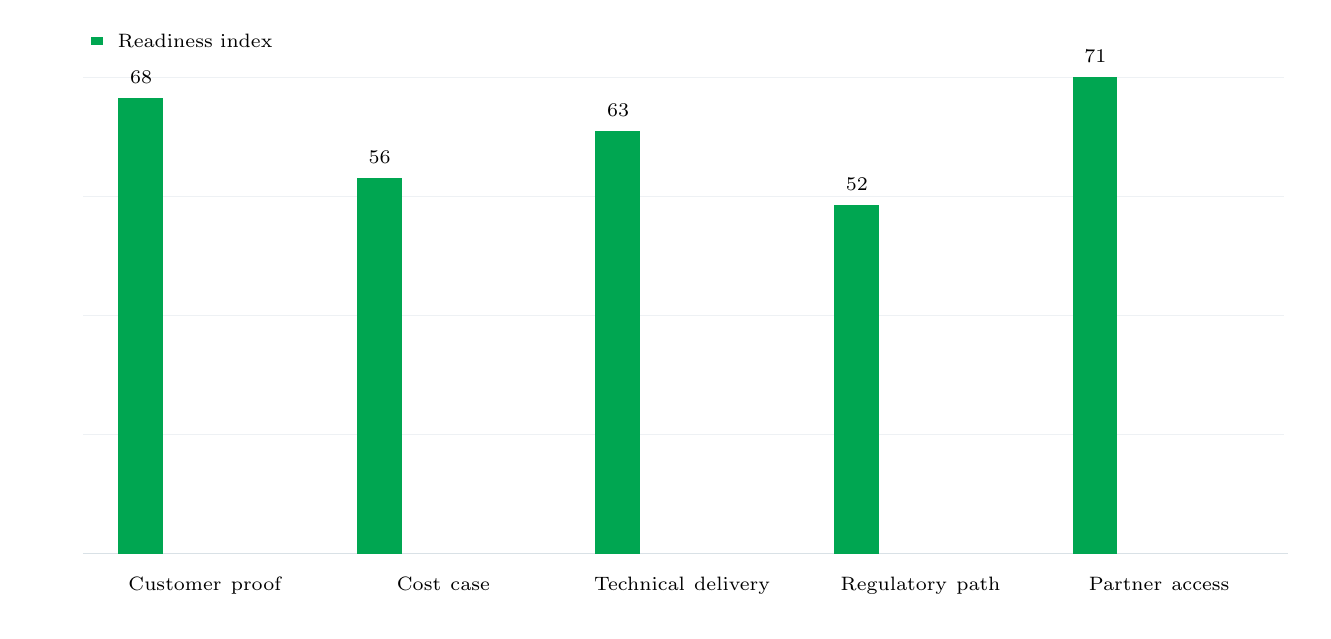
\begin{tikzpicture}[x=1cm,y=1cm]
\path[use as bounding box] (0,0) rectangle (16.20,7.40);
\draw[BOLine] (0.70,0.72) -- (16.00,0.72);
\draw[BOLine,opacity=.45] (0.70,2.23) -- (15.95,2.23);
\draw[BOLine,opacity=.45] (0.70,3.75) -- (15.95,3.75);
\draw[BOLine,opacity=.45] (0.70,5.26) -- (15.95,5.26);
\draw[BOLine,opacity=.45] (0.70,6.77) -- (15.95,6.77);
\fill[BOGreen] (1.15,0.72) rectangle (1.72,6.51);
\node[anchor=south,align=center] at (1.44,6.57) {\scriptsize 68};
\node[anchor=north,align=center,text width=2.79cm] at (2.25,0.55) {\scriptsize Customer proof};
\fill[BOGreen] (4.18,0.72) rectangle (4.75,5.49);
\node[anchor=south,align=center] at (4.47,5.55) {\scriptsize 56};
\node[anchor=north,align=center,text width=2.79cm] at (5.28,0.55) {\scriptsize Cost case};
\fill[BOGreen] (7.21,0.72) rectangle (7.78,6.09);
\node[anchor=south,align=center] at (7.50,6.15) {\scriptsize 63};
\node[anchor=north,align=center,text width=2.79cm] at (8.31,0.55) {\scriptsize Technical delivery};
\fill[BOGreen] (10.24,0.72) rectangle (10.81,5.15);
\node[anchor=south,align=center] at (10.53,5.21) {\scriptsize 52};
\node[anchor=north,align=center,text width=2.79cm] at (11.34,0.55) {\scriptsize Regulatory path};
\fill[BOGreen] (13.27,0.72) rectangle (13.84,6.77);
\node[anchor=south,align=center] at (13.56,6.83) {\scriptsize 71};
\node[anchor=north,align=center,text width=2.79cm] at (14.37,0.55) {\scriptsize Partner access};
\fill[BOGreen] (0.80,7.18) rectangle (0.96,7.28);
\node[anchor=west] at (1.02,7.23) {\scriptsize Readiness index};
\end{tikzpicture}\par\vspace{2pt}
\vspace{4pt}{\footnotesize\color{BOText} The exhibit ranks the proof points a CEO should ask teams to close before moving from monitoring to commitment.}\par
{\scriptsize\color{BOMuted} BlueOcean public-source synthesis.}\par

\clearpage
\label{chap:2}
\noindent\begin{tikzpicture}
\path[use as bounding box] (0,0) rectangle (\linewidth,54mm);
\clip (0,0) rectangle (\linewidth,54mm);
\node[anchor=north west,inner sep=0] at (0,54mm) {
\includegraphics[width=\linewidth]{assets/image-2.png}};
\end{tikzpicture}
\vspace{0pt}
\noindent
\begin{tikzpicture}
\fill[BOGreen] (0,0) rectangle (96mm,1.2pt);
\end{tikzpicture}\par\vspace{8pt}
{\Large\sffamily\bfseries\color{BONavy} Commercial readiness depends on bankability, deliverability and repeat customer proof}\par\vspace{4pt}
{\sffamily\fontsize{15}{20}\selectfont\color{BOGreen} The fusion landscape is characterized by a diversity of approaches, but a convergence is emerging around magnetic confinement, particularly the tokamak and its variants. This convergence reduces technology risk but also.}\par\vspace{9pt}
\begin{multicols}{2}
{\small The fusion landscape is characterized by a diversity of approaches, but a convergence is emerging around magnetic confinement, particularly the tokamak and its variants. This convergence reduces technology risk but also means that differentiation among players is narrowing. Understanding the technological landscape is essential for making informed investment and partnership decisions.}\par
{\small The tokamak, invented in the Soviet Union in the 1950s, remains the most studied and funded fusion concept. ITER, SPARC, and several other private ventures (e.g., Tokamak Energy, General Fusion) use variants of this design. The stellarator, an alternative magnetic confinement device, offers inherent stability but is more complex to build; the Wendelstein 7-X in Germany is the leading example. Inertial confinement fusion, pursued at the National Ignition Facility (NIF), achieved a net energy gain in 2022 but is far from commercial application due to low repetition rates and high costs.}\par
{\small Private ventures are increasingly focusing on compact, high-field tokamaks enabled by high-temperature superconductors (HTS). HTS magnets allow smaller, cheaper reactors with faster development cycles. CFS\BOApos{}s SPARC is the flagship example, but others like Tokamak Energy are also pursuing HTS-based designs. Helion Energy\BOApos{}s field-reversed configuration is a notable outlier, promising direct electricity generation without a steam turbine, which could improve efficiency and reduce costs.}\par
{\small The convergence on magnetic confinement is driven by the physics: magnetic fields are the most efficient way to confine plasma at the temperatures needed for fusion (over 100 million degrees Celsius). Inertial confinement, while successful in achieving ignition, faces daunting engineering challenges for power generation. As a result, the majority of private investment (\$4 billion of the \$5 billion total) has gone to magnetic confinement approaches.}\par
{\small For investors, this convergence means that due diligence should focus on execution capability, intellectual property, and supply chain readiness rather than fundamental physics. The key differentiators will be engineering prowess, cost control, and regulatory strategy. Companies that can demonstrate a clear path to a pilot plant within a decade are likely to attract the most capital.}\par
\end{multicols}
\label{chap:2:end}

\clearpage
{\textcolor{BOGreen}{\scriptsize\bfseries EXHIBIT 2}}\par\vspace{4pt}
{\sffamily\fontsize{17}{21}\selectfont\color{BONavy} Commitment posture should shift as proof matures}\par
{\small\color{BOText} Resource posture for Nuclear Fusion Commercialization: Strategic Implications for Energy Markets and Investment}\par\vspace{6pt}
\noindent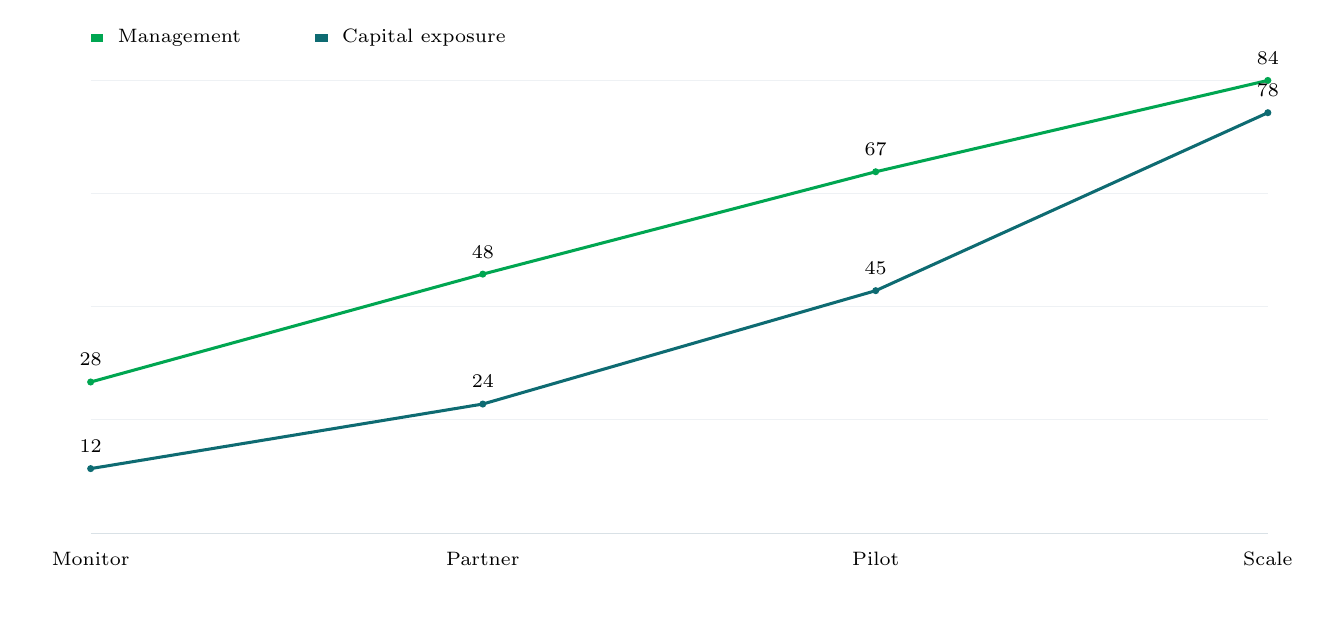
\begin{tikzpicture}[x=1cm,y=1cm]
\path[use as bounding box] (0,0) rectangle (16.20,7.20);
\draw[BOLine] (0.80,0.78) -- (15.75,0.78);
\draw[BOLine,opacity=.45] (0.80,2.22) -- (15.75,2.22);
\draw[BOLine,opacity=.45] (0.80,3.66) -- (15.75,3.66);
\draw[BOLine,opacity=.45] (0.80,5.09) -- (15.75,5.09);
\draw[BOLine,opacity=.45] (0.80,6.53) -- (15.75,6.53);
\draw[BOGreen,line width=1.1pt] (0.80,2.70) -- (5.78,4.07) -- (10.77,5.37) -- (15.75,6.53);
\fill[BOGreen] (0.80,2.70) circle (.045);
\node[anchor=south,align=center] at (0.80,2.78) {\scriptsize 28};
\fill[BOGreen] (5.78,4.07) circle (.045);
\node[anchor=south,align=center] at (5.78,4.15) {\scriptsize 48};
\fill[BOGreen] (10.77,5.37) circle (.045);
\node[anchor=south,align=center] at (10.77,5.45) {\scriptsize 67};
\fill[BOGreen] (15.75,6.53) circle (.045);
\node[anchor=south,align=center] at (15.75,6.61) {\scriptsize 84};
\draw[BOBlue,line width=1.1pt] (0.80,1.60) -- (5.78,2.42) -- (10.77,3.86) -- (15.75,6.12);
\fill[BOBlue] (0.80,1.60) circle (.045);
\node[anchor=south,align=center] at (0.80,1.68) {\scriptsize 12};
\fill[BOBlue] (5.78,2.42) circle (.045);
\node[anchor=south,align=center] at (5.78,2.50) {\scriptsize 24};
\fill[BOBlue] (10.77,3.86) circle (.045);
\node[anchor=south,align=center] at (10.77,3.94) {\scriptsize 45};
\fill[BOBlue] (15.75,6.12) circle (.045);
\node[anchor=south,align=center] at (15.75,6.20) {\scriptsize 78};
\node[anchor=north,align=center,text width=1.8cm] at (0.80,0.66) {\scriptsize Monitor};
\node[anchor=north,align=center,text width=1.8cm] at (5.78,0.66) {\scriptsize Partner};
\node[anchor=north,align=center,text width=1.8cm] at (10.77,0.66) {\scriptsize Pilot};
\node[anchor=north,align=center,text width=1.8cm] at (15.75,0.66) {\scriptsize Scale};
\fill[BOGreen] (0.80,7.02) rectangle (0.96,7.12);
\node[anchor=west] at (1.02,7.07) {\scriptsize Management};
\fill[BOBlue] (3.65,7.02) rectangle (3.81,7.12);
\node[anchor=west] at (3.87,7.07) {\scriptsize Capital exposure};
\end{tikzpicture}\par\vspace{2pt}
\vspace{4pt}{\footnotesize\color{BOText} Capital exposure should lag evidence maturity rather than lead it.}\par
{\scriptsize\color{BOMuted} BlueOcean scenario synthesis.}\par

\clearpage
\label{chap:3}
\noindent\begin{tikzpicture}
\path[use as bounding box] (0,0) rectangle (\linewidth,54mm);
\clip (0,0) rectangle (\linewidth,54mm);
\node[anchor=north west,inner sep=0] at (0,54mm) {
\includegraphics[width=\linewidth]{assets/image-3.png}};
\end{tikzpicture}
\vspace{0pt}
\noindent
\begin{tikzpicture}
\fill[BOGreen] (0,0) rectangle (96mm,1.2pt);
\end{tikzpicture}\par\vspace{8pt}
{\Large\sffamily\bfseries\color{BONavy} Cost, return and timing will determine the real deployment window}\par\vspace{4pt}
{\sffamily\fontsize{15}{20}\selectfont\color{BOGreen} The economic case for fusion rests on its ability to provide clean, baseload power at a cost competitive with other low-carbon sources. Current projections suggest that fusion could achieve a levelized cost of energy (L.}\par\vspace{9pt}
\begin{multicols}{2}
{\small The economic case for fusion rests on its ability to provide clean, baseload power at a cost competitive with other low-carbon sources. Current projections suggest that fusion could achieve a levelized cost of energy (LCOE) of \$50-\$100 per megawatt-hour (MWh) by 2040, but this is highly uncertain and depends on technological progress, scale, and policy support.}\par
{\small For comparison, solar and wind LCOE have fallen dramatically to \$20-\$60/MWh in many markets, and are expected to continue declining. Nuclear fission LCOE is typically \$100-\$150/MWh, with new builds often exceeding \$150/MWh due to construction delays and cost overruns. Fusion must undercut fission and approach renewable costs to be competitive, especially if energy storage costs continue to fall.}\par
{\small Capital expenditure (CAPEX) for a first-of-a-kind fusion plant is estimated at \$5-\$10 billion, similar to a large fission plant. However, fusion plants are expected to have lower fuel costs (tritium and deuterium are abundant) and lower decommissioning costs (no long-lived radioactive waste). Operational costs are uncertain but could be comparable to fission. The key to cost reduction is learning-by-doing: as more plants are built, costs should decline.}\par
{\small Market adoption scenarios vary widely. An optimistic scenario sees fusion providing 10-20\% of global electricity by 2050, driven by aggressive climate policies and successful demonstration plants. A moderate scenario sees 2-5\% penetration, with fusion serving niche markets (e.g., industrial heat, hydrogen production). A pessimistic scenario sees fusion failing to achieve cost parity, with less than 1\% penetration.}\par
{\small The economic viability of fusion is also sensitive to carbon pricing. A carbon price of \$50-\$100 per ton of CO2 would improve fusion\BOApos{}s competitiveness relative to fossil fuels. Without such pricing, fusion may struggle to compete with cheap renewables. Policy support, such as investment tax credits or feed-in tariffs, could accelerate deployment.}\par
\end{multicols}
\label{chap:3:end}

\clearpage
{\textcolor{BOGreen}{\scriptsize\bfseries EXHIBIT 3}}\par\vspace{4pt}
{\sffamily\fontsize{17}{21}\selectfont\color{BONavy} Key risks should be ranked by severity and manageability}\par
{\small\color{BOText} Risk exposure for Nuclear Fusion Commercialization: Strategic Implications for Energy Markets and Investment}\par\vspace{6pt}
\noindent\begin{tikzpicture}[x=1cm,y=1cm]
\path[use as bounding box] (0,0) rectangle (15.60,5.20);
\draw[BOLine] (0.85,0.65) -- (15.10,0.65) -- (15.10,4.60);
\draw[BOLine,dashed] (0.85,2.62) -- (15.10,2.62);
\draw[BOLine,dashed] (7.97,0.65) -- (7.97,4.60);
\fill[BOGreen,opacity=.65] (11.11,3.73) circle (0.24);
\node[anchor=east,align=right,text width=2.55cm] at (10.69,4.12) {\scriptsize Customer demand};
\fill[BOGreen,opacity=.65] (12.25,3.26) circle (0.24);
\node[anchor=east,align=right,text width=2.55cm] at (11.83,3.47) {\scriptsize Cost / ROI};
\fill[BOGreen,opacity=.65] (9.11,3.10) circle (0.20);
\node[anchor=west,align=left,text width=2.55cm] at (9.49,3.13) {\scriptsize Regulation};
\fill[BOGreen,opacity=.65] (9.97,2.78) circle (0.19);
\node[anchor=west,align=left,text width=2.55cm] at (10.34,2.62) {\scriptsize Supply chain};
\fill[BOGreen,opacity=.65] (8.26,2.55) circle (0.17);
\node[anchor=west,align=left,text width=2.55cm] at (8.61,2.21) {\scriptsize Financing};
\node[anchor=north east] at (15.10,0.53) {\scriptsize Severity};
\node[anchor=center,rotate=90] at (0.55,2.62) {\scriptsize Likelihood};
\end{tikzpicture}\par\vspace{2pt}
\vspace{4pt}{\footnotesize\color{BOText} Bubble size indicates the management attention required.}\par
{\scriptsize\color{BOMuted} BlueOcean risk screen.}\par

\clearpage
\label{chap:4}
\noindent\begin{tikzpicture}
\path[use as bounding box] (0,0) rectangle (\linewidth,54mm);
\clip (0,0) rectangle (\linewidth,54mm);
\node[anchor=north west,inner sep=0] at (0,54mm) {
\includegraphics[width=\linewidth]{assets/image-4.png}};
\end{tikzpicture}
\vspace{0pt}
\noindent
\begin{tikzpicture}
\fill[BOGreen] (0,0) rectangle (96mm,1.2pt);
\end{tikzpicture}\par\vspace{8pt}
{\Large\sffamily\bfseries\color{BONavy} Regulation, policy and public acceptance can reset the speed of adoption}\par\vspace{4pt}
{\sffamily\fontsize{15}{20}\selectfont\color{BOGreen} The regulatory landscape for fusion is in its infancy, but progress is being made. The U.S. Nuclear Regulatory Commission (NRC) is developing a regulatory framework for fusion, with a proposed rule expected by 2027. The.}\par\vspace{9pt}
\begin{multicols}{2}
{\small The regulatory landscape for fusion is in its infancy, but progress is being made. The U.S. Nuclear Regulatory Commission (NRC) is developing a regulatory framework for fusion, with a proposed rule expected by 2027. The UK has established a fusion regulatory framework under the Environment Agency. No fusion plant has been licensed yet, but first-of-a-kind licensing is expected by 2030.}\par
{\small Engaging early with regulators can help shape standards and reduce licensing risk. First-mover advantage in regulatory compliance could be significant, as early entrants may influence the development of safety standards and licensing processes.}\par
{\small For capital allocation, the key takeaway is that regulatory engagement should be a priority. Companies that invest in understanding and shaping the regulatory environment will be better positioned to navigate the licensing process and bring fusion plants to market.}\par
{\small For Regulation, policy and public acceptance can reset the speed of adoption, the next useful work is to convert the supporting sources into a short list of claims that would change capital timing, customer exposure or partner posture. Claims that do not change those decisions should stay out of the main narrative.}\par
{\small Policy support, permitting rules, standards and public acceptance affect how quickly an opportunity moves from concept to deployment. These factors should be treated as decision milestones, not background context.}\par
\end{multicols}
\label{chap:4:end}

\clearpage
{\textcolor{BOGreen}{\scriptsize\bfseries EXHIBIT 4}}\par\vspace{4pt}
{\sffamily\fontsize{17}{21}\selectfont\color{BONavy} Diligence workload concentrates in customer, cost and policy proof}\par
{\small\color{BOText} Near-term validation load for Nuclear Fusion Commercialization: Strategic Implications for Energy Markets and Investment}\par\vspace{6pt}
\noindent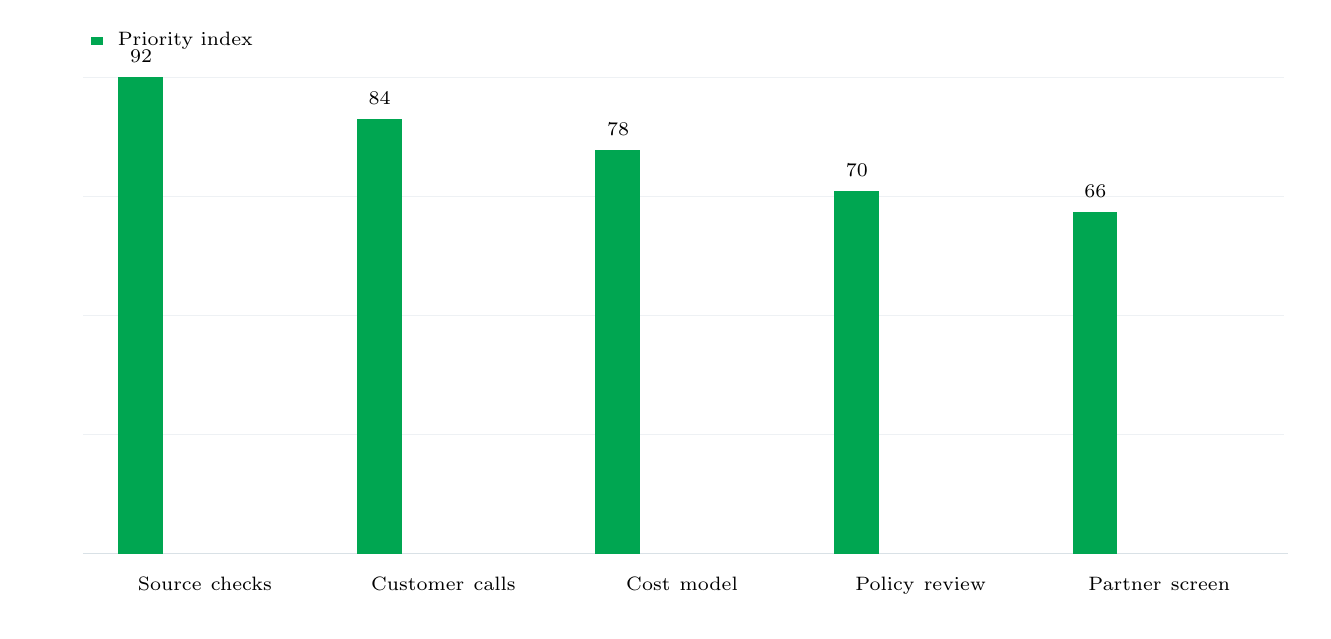
\begin{tikzpicture}[x=1cm,y=1cm]
\path[use as bounding box] (0,0) rectangle (16.20,7.40);
\draw[BOLine] (0.70,0.72) -- (16.00,0.72);
\draw[BOLine,opacity=.45] (0.70,2.23) -- (15.95,2.23);
\draw[BOLine,opacity=.45] (0.70,3.75) -- (15.95,3.75);
\draw[BOLine,opacity=.45] (0.70,5.26) -- (15.95,5.26);
\draw[BOLine,opacity=.45] (0.70,6.77) -- (15.95,6.77);
\fill[BOGreen] (1.15,0.72) rectangle (1.72,6.77);
\node[anchor=south,align=center] at (1.44,6.83) {\scriptsize 92};
\node[anchor=north,align=center,text width=2.79cm] at (2.25,0.55) {\scriptsize Source checks};
\fill[BOGreen] (4.18,0.72) rectangle (4.75,6.24);
\node[anchor=south,align=center] at (4.47,6.30) {\scriptsize 84};
\node[anchor=north,align=center,text width=2.79cm] at (5.28,0.55) {\scriptsize Customer calls};
\fill[BOGreen] (7.21,0.72) rectangle (7.78,5.85);
\node[anchor=south,align=center] at (7.50,5.91) {\scriptsize 78};
\node[anchor=north,align=center,text width=2.79cm] at (8.31,0.55) {\scriptsize Cost model};
\fill[BOGreen] (10.24,0.72) rectangle (10.81,5.32);
\node[anchor=south,align=center] at (10.53,5.38) {\scriptsize 70};
\node[anchor=north,align=center,text width=2.79cm] at (11.34,0.55) {\scriptsize Policy review};
\fill[BOGreen] (13.27,0.72) rectangle (13.84,5.06);
\node[anchor=south,align=center] at (13.56,5.12) {\scriptsize 66};
\node[anchor=north,align=center,text width=2.79cm] at (14.37,0.55) {\scriptsize Partner screen};
\fill[BOGreen] (0.80,7.18) rectangle (0.96,7.28);
\node[anchor=west] at (1.02,7.23) {\scriptsize Priority index};
\end{tikzpicture}\par\vspace{2pt}
\vspace{4pt}{\footnotesize\color{BOText} The most valuable work closes open questions that can change the decision.}\par
{\scriptsize\color{BOMuted} BlueOcean public-source synthesis.}\par

\clearpage
\label{chap:5}
\noindent\begin{tikzpicture}
\path[use as bounding box] (0,0) rectangle (\linewidth,54mm);
\clip (0,0) rectangle (\linewidth,54mm);
\node[anchor=north west,inner sep=0] at (0,54mm) {
\includegraphics[width=\linewidth]{assets/image-5.png}};
\end{tikzpicture}
\vspace{0pt}
\noindent
\begin{tikzpicture}
\fill[BOGreen] (0,0) rectangle (96mm,1.2pt);
\end{tikzpicture}\par\vspace{8pt}
{\Large\sffamily\bfseries\color{BONavy} Supply chain, partners and talent will decide who can act before the market is obvious}\par\vspace{4pt}
{\sffamily\fontsize{15}{20}\selectfont\color{BOGreen} Strategic advantage comes from ecosystem position rather than standalone product capability.}\par\vspace{9pt}
\begin{multicols}{2}
{\small In uncertain markets, early advantage often comes from supply access, partner entry, talent pools and customer learning rather than a single technology claim.}\par
{\small Management should identify which capabilities are scarce and can be secured early: critical supply, engineering delivery, channel partners, service network, financing partners and compliance capacity. Low-cost learning rights can be more valuable than waiting for full market clarity.}\par
{\small Partnerships should create observable proof points. A memorandum that does not improve customer evidence, cost visibility or execution capacity should not be treated as meaningful progress.}\par
{\small For a CEO, Supply chain, partners and talent will decide who can act before the market is obvious matters only if it changes the timing of capital, partner access, customer commitments or risk appetite. The strongest posture is to keep learning close to the business while reserving heavier commitments for proof that can survive investment-committee scrutiny.}\par
{\small For Supply chain, partners and talent will decide who can act before the market is obvious, resource allocation should follow the facts that can change the decision: customer demand, cost position, financing availability, regulatory path and delivery capability. If those facts do not improve, increasing exposure mainly creates strategic lock-in rather than higher conviction.}\par
\end{multicols}
\label{chap:5:end}

\clearpage
{\textcolor{BOGreen}{\scriptsize\bfseries EXHIBIT 5}}\par\vspace{4pt}
{\sffamily\fontsize{17}{21}\selectfont\color{BONavy} Scenario choices should compare attractiveness with readiness}\par
{\small\color{BOText} Strategic option comparison for Nuclear Fusion Commercialization: Strategic Implications for Energy Markets and Investment}\par\vspace{6pt}
{\scriptsize\begin{tabular}{p{38mm}>{\centering\arraybackslash}p{21mm}>{\centering\arraybackslash}p{21mm}>{\centering\arraybackslash}p{21mm}>{\centering\arraybackslash}p{21mm}}
 & {\bfseries Attractiveness} & {\bfseries Readiness} & {\bfseries Confidence} & {\bfseries Capital need} \\
\hline
{\bfseries Nuclear Fusion} & \colorbox{BOGreen}{\textcolor{white}{\strut\hspace{5pt}5\hspace{5pt}}} & \colorbox{BOBlue}{\textcolor{white}{\strut\hspace{5pt}3\hspace{5pt}}} & \colorbox{BOLight}{\textcolor{BOText}{\strut\hspace{5pt}2\hspace{5pt}}} & \colorbox{BOLight}{\textcolor{BOText}{\strut\hspace{5pt}2\hspace{5pt}}} \\
{\bfseries Commercial readiness depends on} & \colorbox{BOGreen}{\textcolor{white}{\strut\hspace{5pt}4\hspace{5pt}}} & \colorbox{BOGreen}{\textcolor{white}{\strut\hspace{5pt}4\hspace{5pt}}} & \colorbox{BOBlue}{\textcolor{white}{\strut\hspace{5pt}3\hspace{5pt}}} & \colorbox{BOBlue}{\textcolor{white}{\strut\hspace{5pt}3\hspace{5pt}}} \\
{\bfseries Cost, return and timing will} & \colorbox{BOGreen}{\textcolor{white}{\strut\hspace{5pt}4\hspace{5pt}}} & \colorbox{BOLight}{\textcolor{BOText}{\strut\hspace{5pt}2\hspace{5pt}}} & \colorbox{BOLight}{\textcolor{BOText}{\strut\hspace{5pt}2\hspace{5pt}}} & \colorbox{BOGreen}{\textcolor{white}{\strut\hspace{5pt}4\hspace{5pt}}} \\
{\bfseries Regulation, policy and public} & \colorbox{BOBlue}{\textcolor{white}{\strut\hspace{5pt}3\hspace{5pt}}} & \colorbox{BOBlue}{\textcolor{white}{\strut\hspace{5pt}3\hspace{5pt}}} & \colorbox{BOBlue}{\textcolor{white}{\strut\hspace{5pt}3\hspace{5pt}}} & \colorbox{BOLight}{\textcolor{BOText}{\strut\hspace{5pt}2\hspace{5pt}}} \\
{\bfseries Supply chain, partners} & \colorbox{BOGreen}{\textcolor{white}{\strut\hspace{5pt}5\hspace{5pt}}} & \colorbox{BOBlue}{\textcolor{white}{\strut\hspace{5pt}3\hspace{5pt}}} & \colorbox{BOBlue}{\textcolor{white}{\strut\hspace{5pt}3\hspace{5pt}}} & \colorbox{BOBlue}{\textcolor{white}{\strut\hspace{5pt}3\hspace{5pt}}} \\
\end{tabular}}\par\vspace{2pt}
\vspace{4pt}{\footnotesize\color{BOText} The matrix ranks where the next validation work should focus.}\par
{\scriptsize\color{BOMuted} BlueOcean qualitative assessment.}\par

\clearpage
\label{chap:6}
\noindent\begin{tikzpicture}
\path[use as bounding box] (0,0) rectangle (\linewidth,54mm);
\clip (0,0) rectangle (\linewidth,54mm);
\node[anchor=north west,inner sep=0] at (0,54mm) {
\includegraphics[width=\linewidth]{assets/image-6.png}};
\end{tikzpicture}
\vspace{0pt}
\noindent
\begin{tikzpicture}
\fill[BOGreen] (0,0) rectangle (96mm,1.2pt);
\end{tikzpicture}\par\vspace{8pt}
{\Large\sffamily\bfseries\color{BONavy} Incumbents should protect near-term economics while preserving long-term options}\par\vspace{4pt}
{\sffamily\fontsize{15}{20}\selectfont\color{BOGreen} The strongest posture is neither aggressive overcommitment nor passive observation.}\par\vspace{9pt}
\begin{multicols}{2}
{\small For incumbent businesses, the task is to protect near-term cash flow and customer relationships while avoiding strategic blindness to a long-term shift. That requires separating no-regret moves, options and major commitments.}\par
{\small No-regret moves include evidence ledgers, customer interviews, policy monitoring, supply-chain scans and small partner discussions. Option moves include pilots, preferential access and minority investments. Major commitments should wait for stronger proof.}\par
{\small This portfolio posture keeps the organization close to the opportunity without locking strategy and capital before the evidence base is ready.}\par
{\small For a CEO, Incumbents should protect near-term economics while preserving long-term options matters only if it changes the timing of capital, partner access, customer commitments or risk appetite. The strongest posture is to keep learning close to the business while reserving heavier commitments for proof that can survive investment-committee scrutiny.}\par
{\small For Incumbents should protect near-term economics while preserving long-term options, resource allocation should follow the facts that can change the decision: customer demand, cost position, financing availability, regulatory path and delivery capability. If those facts do not improve, increasing exposure mainly creates strategic lock-in rather than higher conviction.}\par
\end{multicols}
\label{chap:6:end}

\clearpage
{\textcolor{BOGreen}{\scriptsize\bfseries EXHIBIT 6}}\par\vspace{4pt}
{\sffamily\fontsize{17}{21}\selectfont\color{BONavy} Validation effort shifts from customer proof to policy and partners}\par
{\small\color{BOText} Quarterly validation mix for Nuclear Fusion Commercialization: Strategic Implications for Energy Markets and Investment}\par\vspace{6pt}
\noindent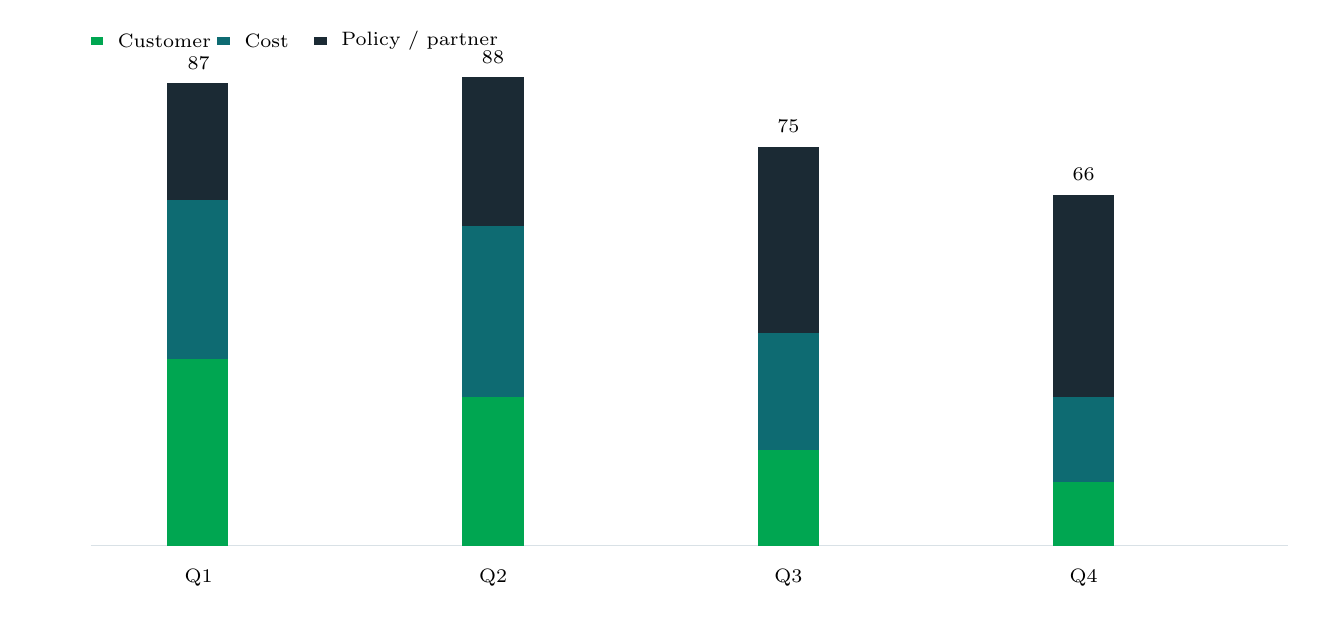
\begin{tikzpicture}[x=1cm,y=1cm]
\path[use as bounding box] (0,0) rectangle (16.20,7.30);
\draw[BOLine] (0.80,0.72) -- (16.00,0.72);
\fill[BOGreen] (1.77,0.72) rectangle (2.55,3.09);
\fill[BOBlue] (1.77,3.09) rectangle (2.55,5.11);
\fill[BONavy] (1.77,5.11) rectangle (2.55,6.60);
\node[anchor=south,align=center] at (2.17,6.65) {\scriptsize 87};
\node[anchor=north,align=center,text width=3.45cm] at (2.17,0.55) {\scriptsize Q1};
\fill[BOGreen] (5.52,0.72) rectangle (6.30,2.61);
\fill[BOBlue] (5.52,2.61) rectangle (6.30,4.78);
\fill[BONavy] (5.52,4.78) rectangle (6.30,6.67);
\node[anchor=south,align=center] at (5.91,6.72) {\scriptsize 88};
\node[anchor=north,align=center,text width=3.45cm] at (5.91,0.55) {\scriptsize Q2};
\fill[BOGreen] (9.27,0.72) rectangle (10.05,1.94);
\fill[BOBlue] (9.27,1.94) rectangle (10.05,3.42);
\fill[BONavy] (9.27,3.42) rectangle (10.05,5.79);
\node[anchor=south,align=center] at (9.66,5.84) {\scriptsize 75};
\node[anchor=north,align=center,text width=3.45cm] at (9.66,0.55) {\scriptsize Q3};
\fill[BOGreen] (13.02,0.72) rectangle (13.80,1.53);
\fill[BOBlue] (13.02,1.53) rectangle (13.80,2.61);
\fill[BONavy] (13.02,2.61) rectangle (13.80,5.18);
\node[anchor=south,align=center] at (13.41,5.23) {\scriptsize 66};
\node[anchor=north,align=center,text width=3.45cm] at (13.41,0.55) {\scriptsize Q4};
\fill[BOGreen] (0.80,7.08) rectangle (0.96,7.18);
\node[anchor=west] at (1.02,7.13) {\scriptsize Customer};
\fill[BOBlue] (2.41,7.08) rectangle (2.57,7.18);
\node[anchor=west] at (2.63,7.13) {\scriptsize Cost};
\fill[BONavy] (3.64,7.08) rectangle (3.80,7.18);
\node[anchor=west] at (3.86,7.13) {\scriptsize Policy / partner};
\end{tikzpicture}\par\vspace{2pt}
\vspace{4pt}{\footnotesize\color{BOText} The validation cadence should improve facts before escalating resource commitment.}\par
{\scriptsize\color{BOMuted} BlueOcean public-source synthesis.}\par

\clearpage
\label{chap:7}
\noindent\begin{tikzpicture}
\path[use as bounding box] (0,0) rectangle (\linewidth,54mm);
\clip (0,0) rectangle (\linewidth,54mm);
\node[anchor=north west,inner sep=0] at (0,54mm) {
\includegraphics[width=\linewidth]{assets/image-7.png}};
\end{tikzpicture}
\vspace{0pt}
\noindent
\begin{tikzpicture}
\fill[BOGreen] (0,0) rectangle (96mm,1.2pt);
\end{tikzpicture}\par\vspace{8pt}
{\Large\sffamily\bfseries\color{BONavy} The management agenda should translate uncertainty into quarterly decision milestones}\par\vspace{4pt}
{\sffamily\fontsize{15}{20}\selectfont\color{BOGreen} The report should end in owners, evidence thresholds and review cadence.}\par\vspace{9pt}
\begin{multicols}{2}
{\small The output should become a quarterly management agenda: every material claim needs an owner, evidence gate, review date and escalation condition.}\par
{\small Near-term work should close source, customer, cost and timeline gaps; medium-term work should test pilots and partners; long-term work should cover capital, M\&A or scaled entry only when decision milestones are met.}\par
{\small If the next evidence review does not improve conviction, management should keep the issue in monitoring mode. If the core metrics move, the topic can be escalated to an investment committee discussion.}\par
{\small For a CEO, The management agenda should translate uncertainty into quarterly decision milestones matters only if it changes the timing of capital, partner access, customer commitments or risk appetite. The strongest posture is to keep learning close to the business while reserving heavier commitments for proof that can survive investment-committee scrutiny.}\par
{\small For The management agenda should translate uncertainty into quarterly decision milestones, resource allocation should follow the facts that can change the decision: customer demand, cost position, financing availability, regulatory path and delivery capability. If those facts do not improve, increasing exposure mainly creates strategic lock-in rather than higher conviction.}\par
\end{multicols}
\label{chap:7:end}

\clearpage
{\textcolor{BOGreen}{\scriptsize\bfseries EXHIBIT 7}}\par\vspace{4pt}
{\sffamily\fontsize{17}{21}\selectfont\color{BONavy} Cost structure must be decomposed before underwriting}\par
{\small\color{BOText} Cost diligence view for Nuclear Fusion Commercialization: Strategic Implications for Energy Markets and Investment}\par\vspace{6pt}
\noindent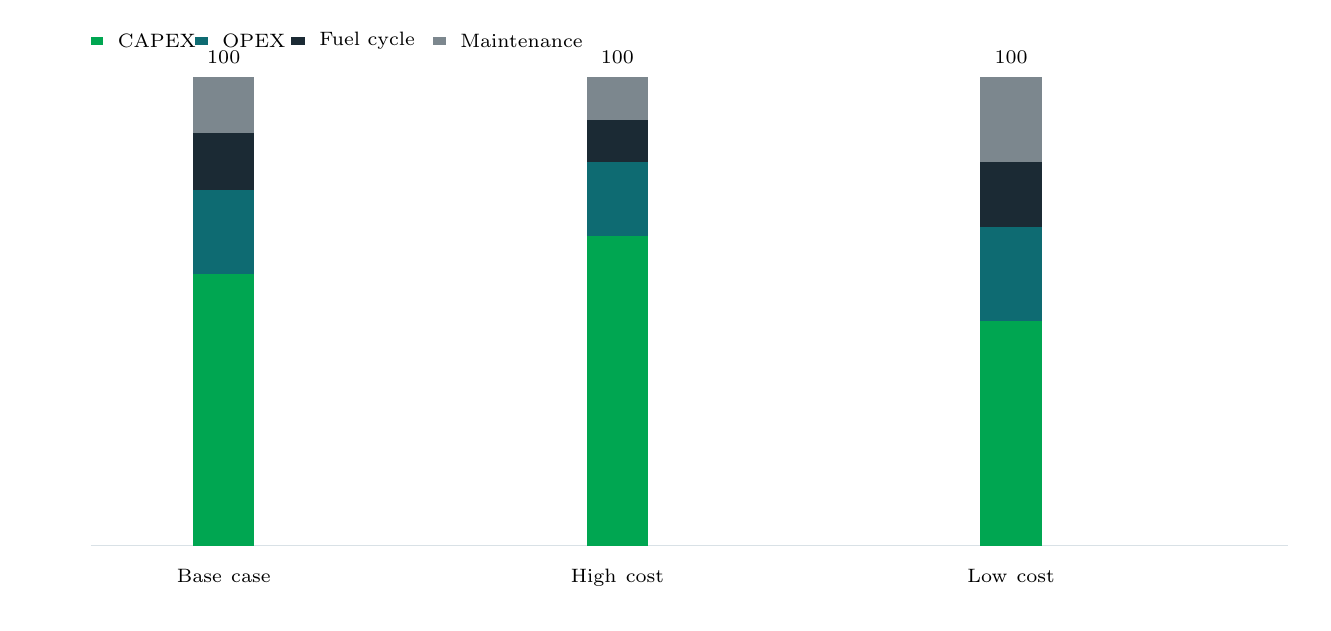
\begin{tikzpicture}[x=1cm,y=1cm]
\path[use as bounding box] (0,0) rectangle (16.20,7.30);
\draw[BOLine] (0.80,0.72) -- (16.00,0.72);
\fill[BOGreen] (2.10,0.72) rectangle (2.88,4.17);
\fill[BOBlue] (2.10,4.17) rectangle (2.88,5.24);
\fill[BONavy] (2.10,5.24) rectangle (2.88,5.96);
\fill[BOMuted] (2.10,5.96) rectangle (2.88,6.67);
\node[anchor=south,align=center] at (2.49,6.72) {\scriptsize 100};
\node[anchor=north,align=center,text width=4.60cm] at (2.49,0.55) {\scriptsize Base case};
\fill[BOGreen] (7.10,0.72) rectangle (7.88,4.65);
\fill[BOBlue] (7.10,4.65) rectangle (7.88,5.60);
\fill[BONavy] (7.10,5.60) rectangle (7.88,6.13);
\fill[BOMuted] (7.10,6.13) rectangle (7.88,6.67);
\node[anchor=south,align=center] at (7.49,6.72) {\scriptsize 100};
\node[anchor=north,align=center,text width=4.60cm] at (7.49,0.55) {\scriptsize High cost};
\fill[BOGreen] (12.10,0.72) rectangle (12.88,3.58);
\fill[BOBlue] (12.10,3.58) rectangle (12.88,4.77);
\fill[BONavy] (12.10,4.77) rectangle (12.88,5.60);
\fill[BOMuted] (12.10,5.60) rectangle (12.88,6.67);
\node[anchor=south,align=center] at (12.49,6.72) {\scriptsize 100};
\node[anchor=north,align=center,text width=4.60cm] at (12.49,0.55) {\scriptsize Low cost};
\fill[BOGreen] (0.80,7.08) rectangle (0.96,7.18);
\node[anchor=west] at (1.02,7.13) {\scriptsize CAPEX};
\fill[BOBlue] (2.12,7.08) rectangle (2.29,7.18);
\node[anchor=west] at (2.35,7.13) {\scriptsize OPEX};
\fill[BONavy] (3.35,7.08) rectangle (3.52,7.18);
\node[anchor=west] at (3.58,7.13) {\scriptsize Fuel cycle};
\fill[BOMuted] (5.15,7.08) rectangle (5.31,7.18);
\node[anchor=west] at (5.37,7.13) {\scriptsize Maintenance};
\end{tikzpicture}\par\vspace{2pt}
\vspace{4pt}{\footnotesize\color{BOText} The chart separates capital, operating and maintenance drivers so management can test which cost lever would change the investment case.}\par
{\scriptsize\color{BOMuted} BlueOcean public-source synthesis.}\par

\clearpage
\label{chap:8}
\noindent\begin{tikzpicture}
\path[use as bounding box] (0,0) rectangle (\linewidth,54mm);
\clip (0,0) rectangle (\linewidth,54mm);
\node[anchor=north west,inner sep=0] at (0,54mm) {
\includegraphics[width=\linewidth]{assets/image-8.png}};
\end{tikzpicture}
\vspace{0pt}
\noindent
\begin{tikzpicture}
\fill[BOGreen] (0,0) rectangle (96mm,1.2pt);
\end{tikzpicture}\par\vspace{8pt}
{\Large\sffamily\bfseries\color{BONavy} Decision-moving facts matter more than market noise}\par\vspace{4pt}
{\sffamily\fontsize{15}{20}\selectfont\color{BOGreen} The most useful monitoring lens focuses on customers, costs, regulation, competitors and financing.}\par\vspace{9pt}
\begin{multicols}{2}
{\small For leadership teams, management should not treat media attention, financing announcements or single technical claims as decision signals on their own. More useful signals include customer procurement, cost movement, regulatory clarity, competitor commitments and financing terms.}\par
{\small Each signal should map to an action: keep monitoring, start a pilot, expand a partnership, pause commitment or escalate to the board.}\par
{\small That discipline turns uncertainty into a manageable operating rhythm rather than a swing between optimism and caution.}\par
{\small For a CEO, Decision-moving facts matter more than market noise matters only if it changes the timing of capital, partner access, customer commitments or risk appetite. The strongest posture is to keep learning close to the business while reserving heavier commitments for proof that can survive investment-committee scrutiny.}\par
{\small For Decision-moving facts matter more than market noise, resource allocation should follow the facts that can change the decision: customer demand, cost position, financing availability, regulatory path and delivery capability. If those facts do not improve, increasing exposure mainly creates strategic lock-in rather than higher conviction.}\par
\end{multicols}
\label{chap:8:end}

\clearpage
{\textcolor{BOGreen}{\scriptsize\bfseries EXHIBIT 8}}\par\vspace{4pt}
{\sffamily\fontsize{17}{21}\selectfont\color{BONavy} Timeline confidence falls as milestones move from lab to grid}\par
{\small\color{BOText} Milestone confidence for Nuclear Fusion Commercialization: Strategic Implications for Energy Markets and Investment}\par\vspace{6pt}
\noindent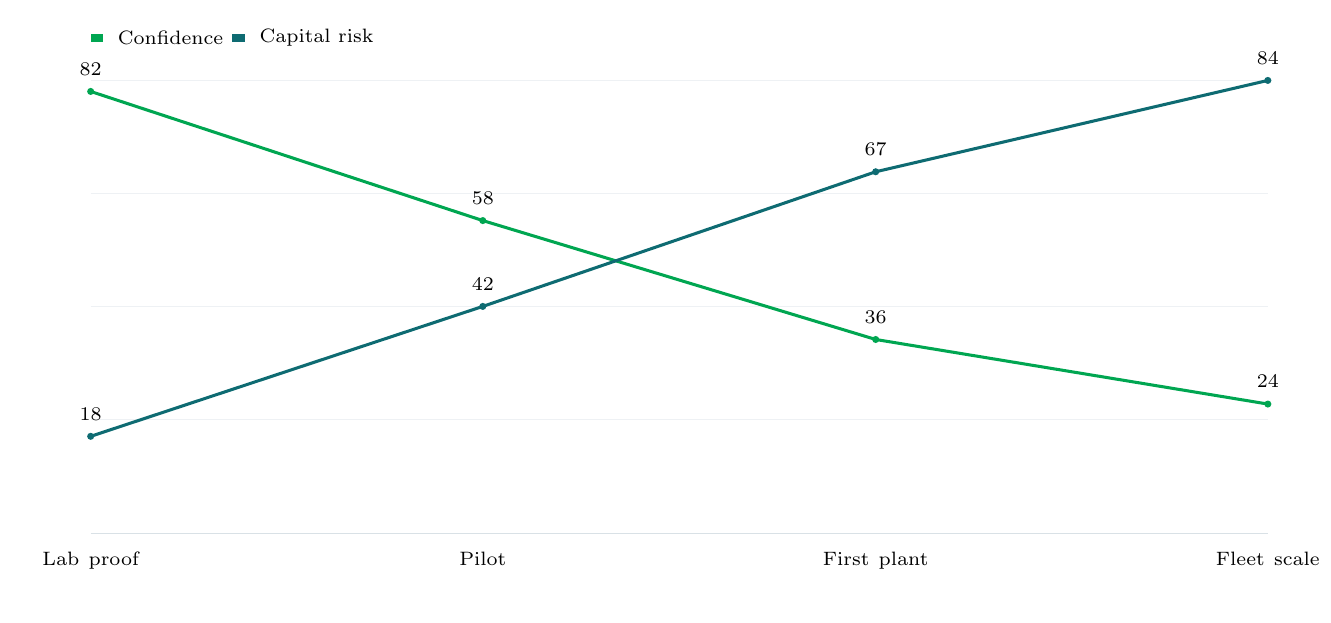
\begin{tikzpicture}[x=1cm,y=1cm]
\path[use as bounding box] (0,0) rectangle (16.20,7.20);
\draw[BOLine] (0.80,0.78) -- (15.75,0.78);
\draw[BOLine,opacity=.45] (0.80,2.22) -- (15.75,2.22);
\draw[BOLine,opacity=.45] (0.80,3.66) -- (15.75,3.66);
\draw[BOLine,opacity=.45] (0.80,5.09) -- (15.75,5.09);
\draw[BOLine,opacity=.45] (0.80,6.53) -- (15.75,6.53);
\draw[BOGreen,line width=1.1pt] (0.80,6.39) -- (5.78,4.75) -- (10.77,3.24) -- (15.75,2.42);
\fill[BOGreen] (0.80,6.39) circle (.045);
\node[anchor=south,align=center] at (0.80,6.47) {\scriptsize 82};
\fill[BOGreen] (5.78,4.75) circle (.045);
\node[anchor=south,align=center] at (5.78,4.83) {\scriptsize 58};
\fill[BOGreen] (10.77,3.24) circle (.045);
\node[anchor=south,align=center] at (10.77,3.32) {\scriptsize 36};
\fill[BOGreen] (15.75,2.42) circle (.045);
\node[anchor=south,align=center] at (15.75,2.50) {\scriptsize 24};
\draw[BOBlue,line width=1.1pt] (0.80,2.01) -- (5.78,3.66) -- (10.77,5.37) -- (15.75,6.53);
\fill[BOBlue] (0.80,2.01) circle (.045);
\node[anchor=south,align=center] at (0.80,2.09) {\scriptsize 18};
\fill[BOBlue] (5.78,3.66) circle (.045);
\node[anchor=south,align=center] at (5.78,3.74) {\scriptsize 42};
\fill[BOBlue] (10.77,5.37) circle (.045);
\node[anchor=south,align=center] at (10.77,5.45) {\scriptsize 67};
\fill[BOBlue] (15.75,6.53) circle (.045);
\node[anchor=south,align=center] at (15.75,6.61) {\scriptsize 84};
\node[anchor=north,align=center,text width=1.8cm] at (0.80,0.66) {\scriptsize Lab proof};
\node[anchor=north,align=center,text width=1.8cm] at (5.78,0.66) {\scriptsize Pilot};
\node[anchor=north,align=center,text width=1.8cm] at (10.77,0.66) {\scriptsize First plant};
\node[anchor=north,align=center,text width=1.8cm] at (15.75,0.66) {\scriptsize Fleet scale};
\fill[BOGreen] (0.80,7.02) rectangle (0.96,7.12);
\node[anchor=west] at (1.02,7.07) {\scriptsize Confidence};
\fill[BOBlue] (2.60,7.02) rectangle (2.76,7.12);
\node[anchor=west] at (2.82,7.07) {\scriptsize Capital risk};
\end{tikzpicture}\par\vspace{2pt}
\vspace{4pt}{\footnotesize\color{BOText} Decision confidence should be staged by milestone maturity.}\par
{\scriptsize\color{BOMuted} BlueOcean milestone assessment.}\par

\clearpage
{\textcolor{BOGreen}{\scriptsize\bfseries EXHIBIT 9}}\par\vspace{4pt}
{\sffamily\fontsize{17}{21}\selectfont\color{BONavy} Partner options differ on learning value and capital exposure}\par
{\small\color{BOText} Where-to-play option view for Nuclear Fusion Commercialization: Strategic Implications for Energy Markets and Investment}\par\vspace{6pt}
{\scriptsize\begin{tabular}{p{38mm}>{\centering\arraybackslash}p{21mm}>{\centering\arraybackslash}p{21mm}>{\centering\arraybackslash}p{21mm}>{\centering\arraybackslash}p{21mm}}
 & {\bfseries Learning} & {\bfseries Control} & {\bfseries Capital need} & {\bfseries Reversibility} \\
\hline
{\bfseries Direct equity} & \colorbox{BOGreen}{\textcolor{white}{\strut\hspace{5pt}5\hspace{5pt}}} & \colorbox{BOGreen}{\textcolor{white}{\strut\hspace{5pt}4\hspace{5pt}}} & \colorbox{BOLight}{\textcolor{BOText}{\strut\hspace{5pt}2\hspace{5pt}}} & \colorbox{BOLight}{\textcolor{BOText}{\strut\hspace{5pt}2\hspace{5pt}}} \\
{\bfseries Corporate venture} & \colorbox{BOGreen}{\textcolor{white}{\strut\hspace{5pt}4\hspace{5pt}}} & \colorbox{BOBlue}{\textcolor{white}{\strut\hspace{5pt}3\hspace{5pt}}} & \colorbox{BOBlue}{\textcolor{white}{\strut\hspace{5pt}3\hspace{5pt}}} & \colorbox{BOBlue}{\textcolor{white}{\strut\hspace{5pt}3\hspace{5pt}}} \\
{\bfseries Offtake option} & \colorbox{BOBlue}{\textcolor{white}{\strut\hspace{5pt}3\hspace{5pt}}} & \colorbox{BOLight}{\textcolor{BOText}{\strut\hspace{5pt}2\hspace{5pt}}} & \colorbox{BOGreen}{\textcolor{white}{\strut\hspace{5pt}4\hspace{5pt}}} & \colorbox{BOGreen}{\textcolor{white}{\strut\hspace{5pt}4\hspace{5pt}}} \\
{\bfseries Supplier JV} & \colorbox{BOGreen}{\textcolor{white}{\strut\hspace{5pt}4\hspace{5pt}}} & \colorbox{BOGreen}{\textcolor{white}{\strut\hspace{5pt}4\hspace{5pt}}} & \colorbox{BOLight}{\textcolor{BOText}{\strut\hspace{5pt}2\hspace{5pt}}} & \colorbox{BOLight}{\textcolor{BOText}{\strut\hspace{5pt}2\hspace{5pt}}} \\
{\bfseries R\&D consortium} & \colorbox{BOBlue}{\textcolor{white}{\strut\hspace{5pt}3\hspace{5pt}}} & \colorbox{BOLight}{\textcolor{BOText}{\strut\hspace{5pt}2\hspace{5pt}}} & \colorbox{BOGreen}{\textcolor{white}{\strut\hspace{5pt}5\hspace{5pt}}} & \colorbox{BOGreen}{\textcolor{white}{\strut\hspace{5pt}5\hspace{5pt}}} \\
\end{tabular}}\par\vspace{2pt}
\vspace{4pt}{\footnotesize\color{BOText} The best early posture maximizes learning without forcing irreversible capital exposure.}\par
{\scriptsize\color{BOMuted} BlueOcean option synthesis.}\par

\clearpage
{\textcolor{BOGreen}{\scriptsize\bfseries EXHIBIT 10}}\par\vspace{4pt}
{\sffamily\fontsize{17}{21}\selectfont\color{BONavy} Evidence maturity varies sharply by claim type}\par
{\small\color{BOText} Claim maturity for Nuclear Fusion Commercialization: Strategic Implications for Energy Markets and Investment}\par\vspace{6pt}
\noindent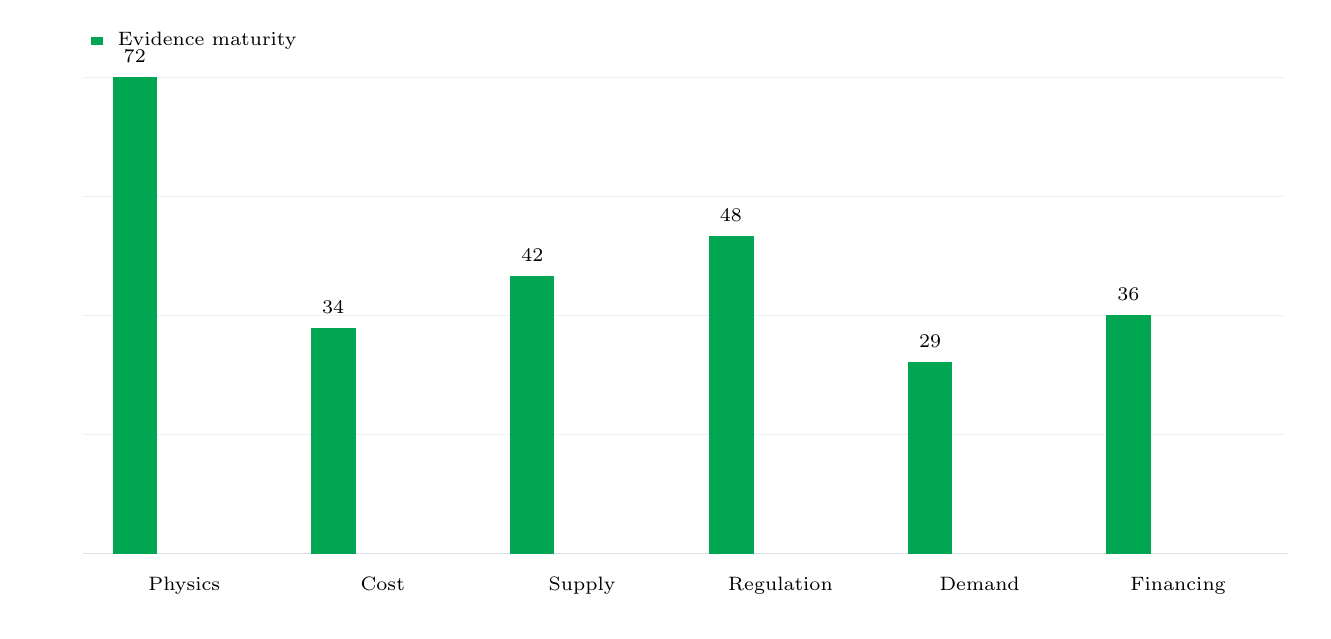
\begin{tikzpicture}[x=1cm,y=1cm]
\path[use as bounding box] (0,0) rectangle (16.20,7.40);
\draw[BOLine] (0.70,0.72) -- (16.00,0.72);
\draw[BOLine,opacity=.45] (0.70,2.23) -- (15.95,2.23);
\draw[BOLine,opacity=.45] (0.70,3.75) -- (15.95,3.75);
\draw[BOLine,opacity=.45] (0.70,5.26) -- (15.95,5.26);
\draw[BOLine,opacity=.45] (0.70,6.77) -- (15.95,6.77);
\fill[BOGreen] (1.08,0.72) rectangle (1.64,6.77);
\node[anchor=south,align=center] at (1.36,6.83) {\scriptsize 72};
\node[anchor=north,align=center,text width=2.32cm] at (1.99,0.55) {\scriptsize Physics};
\fill[BOGreen] (3.60,0.72) rectangle (4.17,3.58);
\node[anchor=south,align=center] at (3.88,3.64) {\scriptsize 34};
\node[anchor=north,align=center,text width=2.32cm] at (4.51,0.55) {\scriptsize Cost};
\fill[BOGreen] (6.13,0.72) rectangle (6.69,4.25);
\node[anchor=south,align=center] at (6.41,4.31) {\scriptsize 42};
\node[anchor=north,align=center,text width=2.32cm] at (7.04,0.55) {\scriptsize Supply};
\fill[BOGreen] (8.65,0.72) rectangle (9.22,4.75);
\node[anchor=south,align=center] at (8.93,4.81) {\scriptsize 48};
\node[anchor=north,align=center,text width=2.32cm] at (9.56,0.55) {\scriptsize Regulation};
\fill[BOGreen] (11.18,0.72) rectangle (11.74,3.16);
\node[anchor=south,align=center] at (11.46,3.22) {\scriptsize 29};
\node[anchor=north,align=center,text width=2.32cm] at (12.09,0.55) {\scriptsize Demand};
\fill[BOGreen] (13.70,0.72) rectangle (14.27,3.75);
\node[anchor=south,align=center] at (13.98,3.81) {\scriptsize 36};
\node[anchor=north,align=center,text width=2.32cm] at (14.61,0.55) {\scriptsize Financing};
\fill[BOGreen] (0.80,7.18) rectangle (0.96,7.28);
\node[anchor=west] at (1.02,7.23) {\scriptsize Evidence maturity};
\end{tikzpicture}\par\vspace{2pt}
\vspace{4pt}{\footnotesize\color{BOText} Management can use the maturity gap to decide which claims support action today and which require a separate diligence workstream.}\par
{\scriptsize\color{BOMuted} BlueOcean public-source synthesis.}\par

\clearpage
{\sffamily\fontsize{20}{25}\selectfont\color{BONavy} About the research}\par\vspace{6pt}
\vspace{2pt}{\color{BOBright}\rule{\linewidth}{1pt}}\vspace{5pt}
{\footnotesize\color{BOMuted} This report has been prepared for strategy discussion and executive decision support. It is not investment, legal, tax, audit or valuation advice. Market estimates, forecasts and scenarios are directional and should be independently validated before they are used for investment, financing, transaction, regulatory or operational decisions. Forward-looking views may change as technology, policy, financing, regulation, competition, supply chains and macro conditions evolve. Recipients should perform their own diligence and treat this report as one input into a broader decision process.}


\clearpage
\thispagestyle{empty}
\begin{tikzpicture}[remember picture,overlay]
\node[anchor=south west,inner sep=0] at (current page.south west) {
\includegraphics[width=\paperwidth,height=\paperheight]{assets/cover-ai.png}};
\fill[black,opacity=.45] (current page.south west) rectangle (current page.north east);
\node[anchor=south east] at ([xshift=-11mm,yshift=10mm]current page.south east) {\sffamily\bfseries\Large\color{white} BlueOcean};
\end{tikzpicture}

\end{document}
